\documentclass[xcolor=svgnames]{beamer}
\usetheme{Singapore}
\setbeamertemplate{footline}[frame number]
\setbeamertemplate{navigation symbols}{}
\setbeamertemplate{itemize item}[triangle]
\setbeamertemplate{itemize subitem}[ball]


\usepackage{amssymb}



\usepackage{tikz}
\usetikzlibrary{arrows,shapes,positioning,calc, shapes.geometric}

\usepackage{listings}
\lstset{
	%  %行号
	%  %numbers=left,
	%  %背景框
	%  %framexleftmargin=10mm,
	%  %frame=none,
	%  %背景色
	%  %backgroundcolor=\color[rgb]{1,1,0.76},
	%  %样式
	keywordstyle=\color{blue}\bfseries,
	%  identifierstyle=\bf,
	%  numberstyle=\color[RGB]{0,192,192}, %行号的样式
	commentstyle=\it\color[RGB]{0,96,96},
	stringstyle=\rmfamily\slshape\color[RGB]{128,0,0},
	%  %显示空格
	%  %showstringspaces=false,
	basicstyle=\ttfamily\scriptsize,
	columns=flexible, %修正大写字母间距过小
	breaklines=true, %对过长的代码自动换行
	%  morekeywords={BEGIN}
}

\definecolor{diffstart}{named}{Grey}
\definecolor{diffincl}{rgb}{0, 0.35, 0}
\definecolor{diffrem}{rgb}{0.72, 0, 0}
\lstdefinelanguage{diff}{
	%basicstyle=\ttfamily\small,
	morecomment=[f][\color{diffstart}]{@@},
	morecomment=[f][\color{diffincl}]{+\ },
	morecomment=[f][\color{diffrem}]{-\ },
}


\usepackage[group-separator={,},group-minimum-digits={3}]{siunitx}


\usepackage{makecell}
\usepackage{caption}
\usepackage{subcaption}
\usepackage{graphicx}

\newcommand{\code}[1]{\texttt{#1}}

\title{Identification of Functional Implementation in Conventional Applications and Transformation to Smart Contracts}
\author{Qiqi Gu\\P0907870}
\institute{%
\tikz[baseline, inner sep=0pt, remember picture]{\node [anchor=base, baseline, inner sep=0pt, align=center] (mpi text)
	{School of Applied Sciences \\ Macao Polytechnic Institute, Macao SAR, China};
}%
}
\date{March 2, 2022}

\parskip=20pt

\begin{document}
\newcommand{\etal}[1]{#1~{\it et al.}}


\tikzstyle{process} = [rectangle, draw=black, inner sep=0.1cm, text centered, align=center]
\tikzstyle{arrow} = [thick, ->, >=stealth]

{
\usebackgroundtemplate{
\includegraphics[height=\paperheight]{background.jpg}}%

\begin{frame}[plain]
	\maketitle

	\begin{tikzpicture}[overlay, remember picture]
	\node[inner sep=0pt, left=0.2cm of mpi text]{
\includegraphics[width=1.2cm]{mpi-logo.png}};
	\end{tikzpicture}
\end{frame}
}

\begin{frame}{Outline}
	\tableofcontents
\end{frame}

\section{Introduction}
\begin{frame}{Smart Contracts}
\begin{itemize}
\item A smart contract is a program running on a blockchain platform.
\item Using smart contracts has many advantages, e.g., reduce the need of trust, reduce enforcement costs.
\item Businesses often use smart contracts as a signed contract or an agreement to regulate the stakeholders~[].
\item<2-> It is difficult to implement smart contracts correctly from the scratch~[].
\end{itemize}
\end{frame}

\begin{frame}{Using Smart Contracts}

\begin{itemize}
\item Businesses already use conventional software to help deal with their business logic.
\item Some of these software are open source and hosted online.
\item We believe it is ideal to transform these applications into smart contracts.
\end{itemize}

\end{frame}

\begin{frame}[t]{Transformation}
\tikzstyle{process} = [rectangle, draw=black, inner sep=0.1cm, text centered, align=center]
\tikzstyle{arrow} = [thick, ->, >=stealth]

\begin{figure}
\centering

\begin{tikzpicture}[remember picture]
\onslide<1,2>{
\node (req) [process] {Requirement Documents};
\node (sc1) [process, below=of req] {Smart Contract};
\draw [arrow] (req) -- (sc1);
}

\onslide<1,3>{
\node (impl) [process, right=of req, xshift=1.5cm] {Source Code};
\node (sc2) [process, below=of impl] {Smart Contract};
\draw [arrow] (impl) -- (sc2);
}
\end{tikzpicture}
\end{figure}

\only<2>{
{\color{Green} \checkmark} Requirement documents capture raw information.

{\color{red} \texttimes} Open source projects typically do not publish such documents.
}

\only<3>{
{\color{Green} \checkmark} Application source code are widely available.

{\color{red} \texttimes} The code may contain too many details and noises.
}

\end{frame}


\begin{frame}{Identification and Transformation}

\begin{enumerate}
\item Identify which conventional applications are transformable

\item Implement algorithms to transform these applications to smart contracts
\end{enumerate}
\end{frame}


\section{Background}
\begin{frame}[t]{Blockchain Platforms}
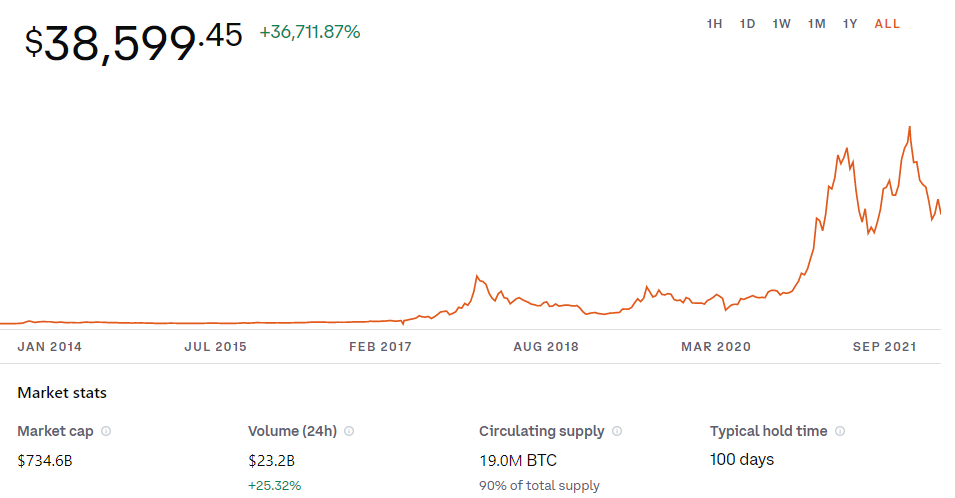
\includegraphics[width=0.9\linewidth]{bitcoin-price}

Market cap of BitCoin reached \$780 billion in January 2022.

The Taproot upgrade took place in November 2021 enabled Bitcoin to execute smart contracts in the core layer.
\end{frame}

\begin{frame}[t]{Blockchain Platforms}
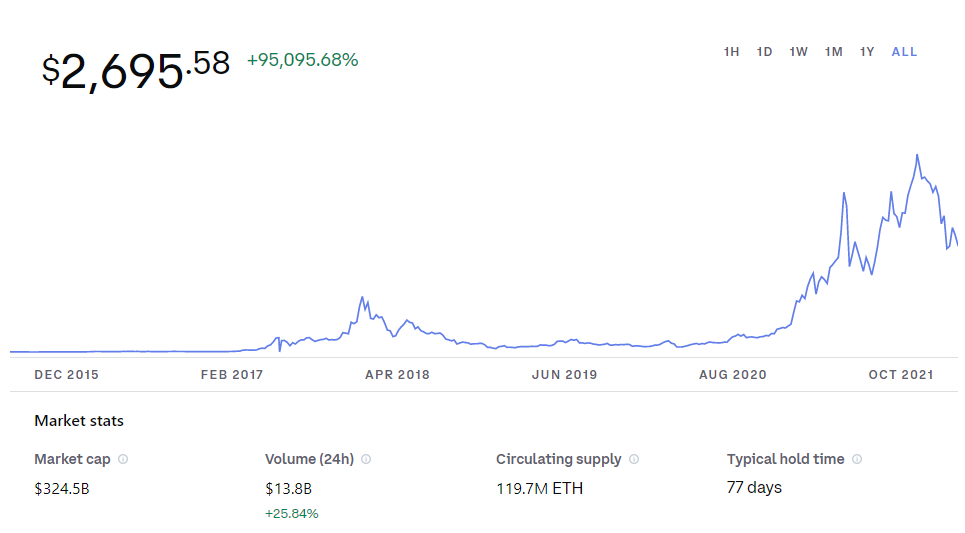
\includegraphics[width=0.9\linewidth]{ethereum-price}

Ethereum is the second largest blockchain platform with market cap of \$360 billion.

It has more mature support of smart contract.
\end{frame}


\begin{frame}{Permissioning of Blockchain Platforms}

\begin{table}
\small
%\setlength\tabcolsep{10pt}
\renewcommand*{\arraystretch}{2}
\begin{tabular}{ll}
Permissionless                                                              & Permissioned                                                \\ \hline
\makecell[l]{Everyone can view the transaction data, \\make transactions, or send queries.} & \makecell[l]{A central authority determines \\who can join the blockchain.} \\
Bitcoin, Ethereum                                                           & \onslide<2->{Hyperledger Fabric}                                          \\
\end{tabular}
\end{table}

\end{frame}

\begin{frame}
\frametitle{

\includegraphics[height=1cm]{hyperledgerfoundation_horizontal-dark.png}
\qquad
\onslide<2->{
\includegraphics[height=1.1cm]{Hyperledger_Fabric_Logo.png}}
}

\begin{itemize}
\item Hyperledger is an umbrella project of open source blockchains and related tools.
\begin{itemize}
\item started in December 2015 by the Linux Foundation
\item gets consistent contributions from IBM, Intel, and so on.
\end{itemize}

\item<2-> In Hyperledger, Fabric is the most developed platform.
\begin{itemize}
\item run smart contracts developed in Java, JavaScript, or NodeJS language
\item preferred by businesses
\end{itemize}
\end{itemize}
\end{frame}


\begin{frame}[t]{Smart Contracts vs.\ DApp}

\begin{itemize}
\item DApp is short for decentralized application.
\begin{onlyenv}<1>
\begin{enumerate}
\item open source. There is no entity controlling the application. Its data are stored in a public blockchain.
\item has tokens to reward user participation. Users spend tokens to interact with the application.
\item be changed in response to consensus of its users~[]
\end{enumerate}
\end{onlyenv}

\item<2-> Development of DApp

\begin{onlyenv}<2>
\begin{figure}
\centering
\begin{tikzpicture}[node distance=0.5cm and 1cm]
\node (whitepaper) [process] {release whitepaper};
\node (program) [process, below=of whitepaper] {release reference program \\for mining or interaction};
\node (mine) [process, below=of program] {mine or stake};
\node (proposals) [process, below=of mine] {write improvement proposals};


\node (whitepaper-icon) [left=of whitepaper] {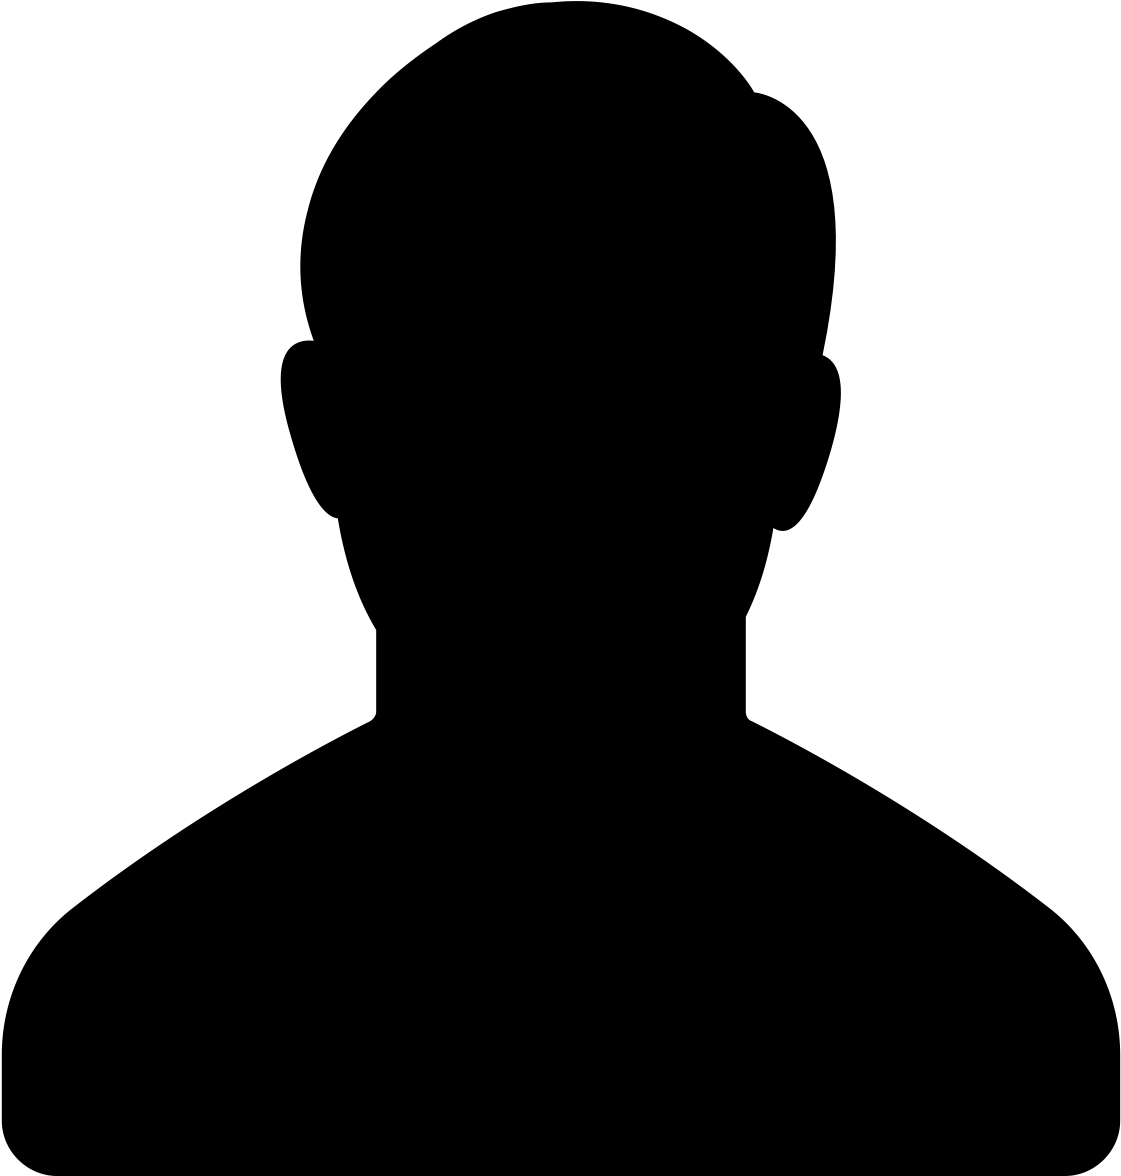
\includegraphics[width=0.5cm]{unknown-person.png}};

\node (program-icon) [opacity=0.9] at (whitepaper-icon |- program) {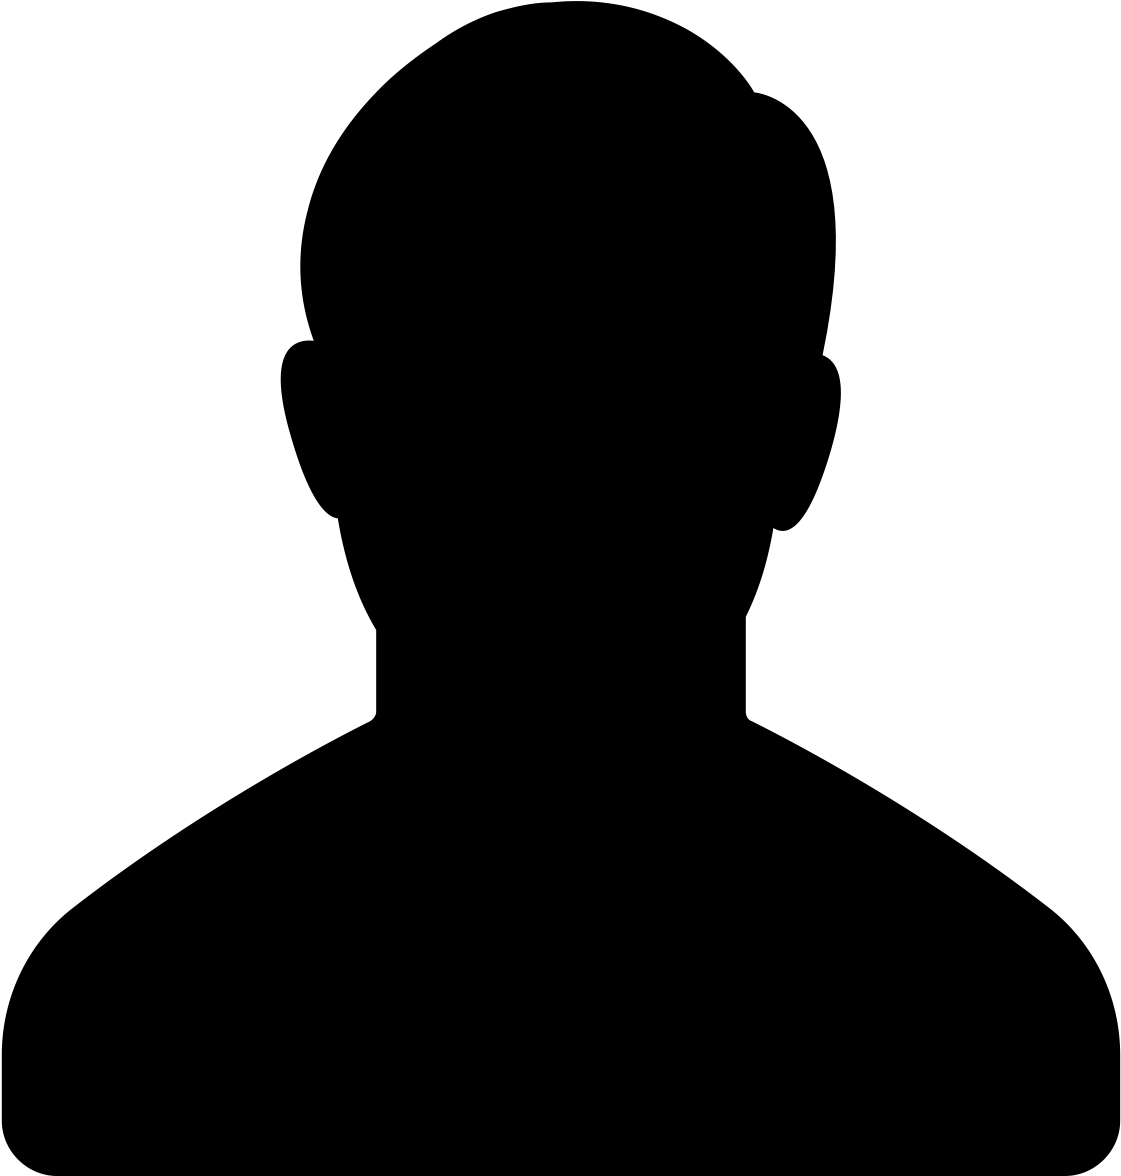
\includegraphics[width=0.5cm]{unknown-person.png}};
\node                [opacity=0.1] at (whitepaper-icon |- program) {
\includegraphics[width=0.5cm]{worldwide.png}};

\node (mine-icon) [opacity=0.7] at (program-icon |- mine) {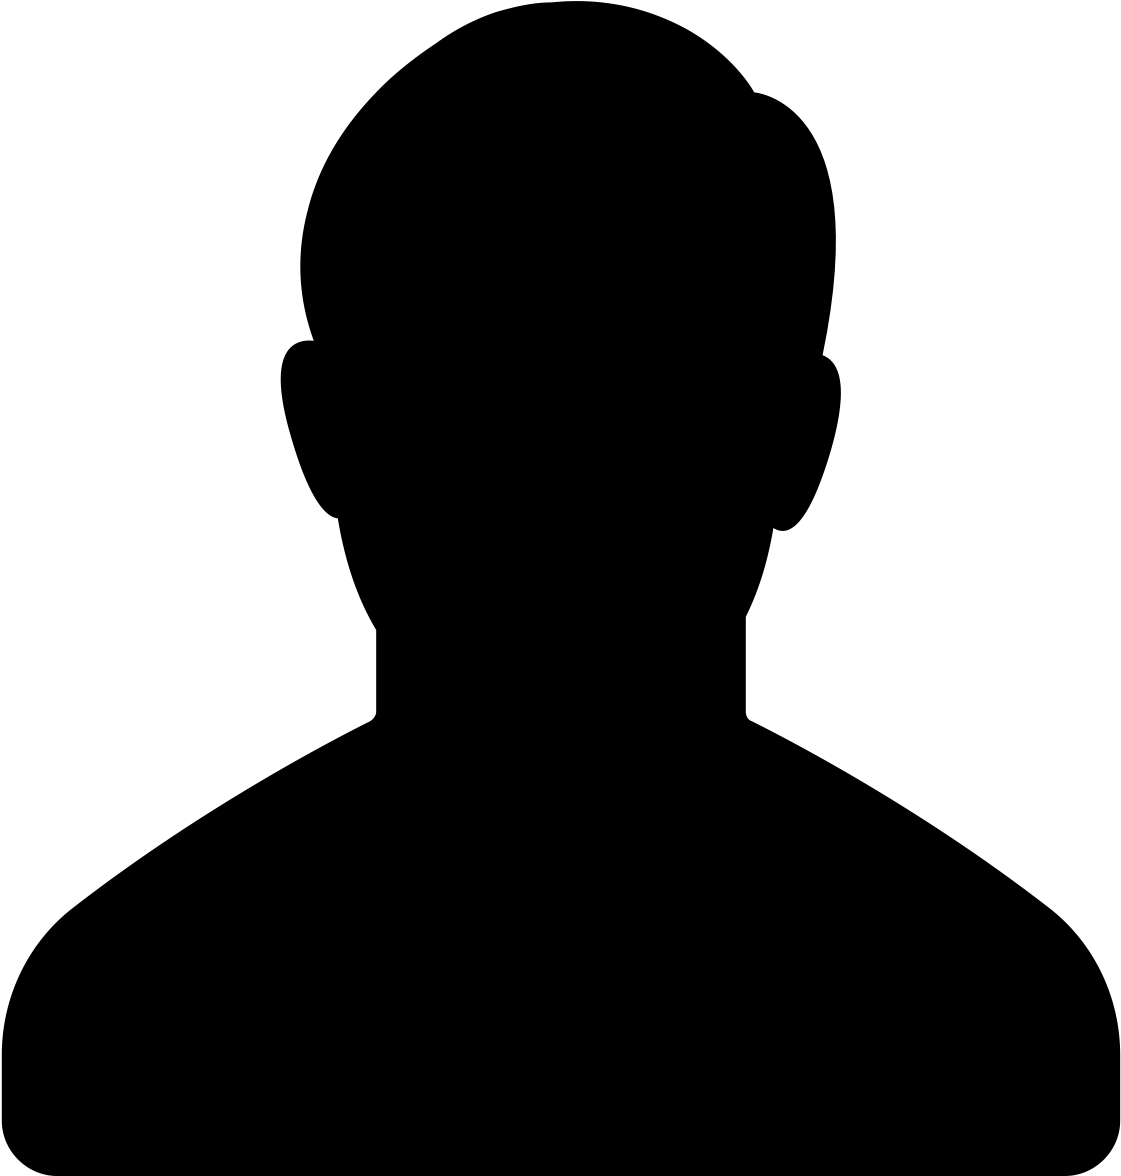
\includegraphics[width=0.5cm]{unknown-person.png}};
\node             [opacity=0.7] at (program-icon |- mine) {
\includegraphics[width=0.5cm]{worldwide.png}};

\node (proposals-icon) at (mine-icon |- proposals) {
\includegraphics[width=0.5cm]{worldwide.png}};

\draw [arrow] (whitepaper) -- (program);
\draw [arrow] (program) -- (mine);
\draw [arrow] (mine) -- (proposals);

\node (centralized) [right=of whitepaper.north east, anchor=south west, xshift=-0.5cm] {\color{DarkViolet} centralized};
\node (decentralized) [anchor=north] at (centralized |- proposals.south) {\color{DeepSkyBlue} decentralized};
\path[shade, top color=DarkViolet, bottom color=DeepSkyBlue] ([xshift=-0.1cm]centralized.south) rectangle ([xshift=0.1cm]decentralized.north);
\end{tikzpicture}
\end{figure}
\end{onlyenv}

\item<3-> A DApp can be a protocol or a group of smart contracts.
\item<4-> In this project we mainly grapple one or a couple of smart contracts, and we do not zero in the decentralization part.
\end{itemize}

\end{frame}


\begin{frame}[t]{RM2PT}
\etal{Yang}~[] proposed a tool, RM2PT, to transform a requirement document into a Java desktop program.
\onslide*<2>{
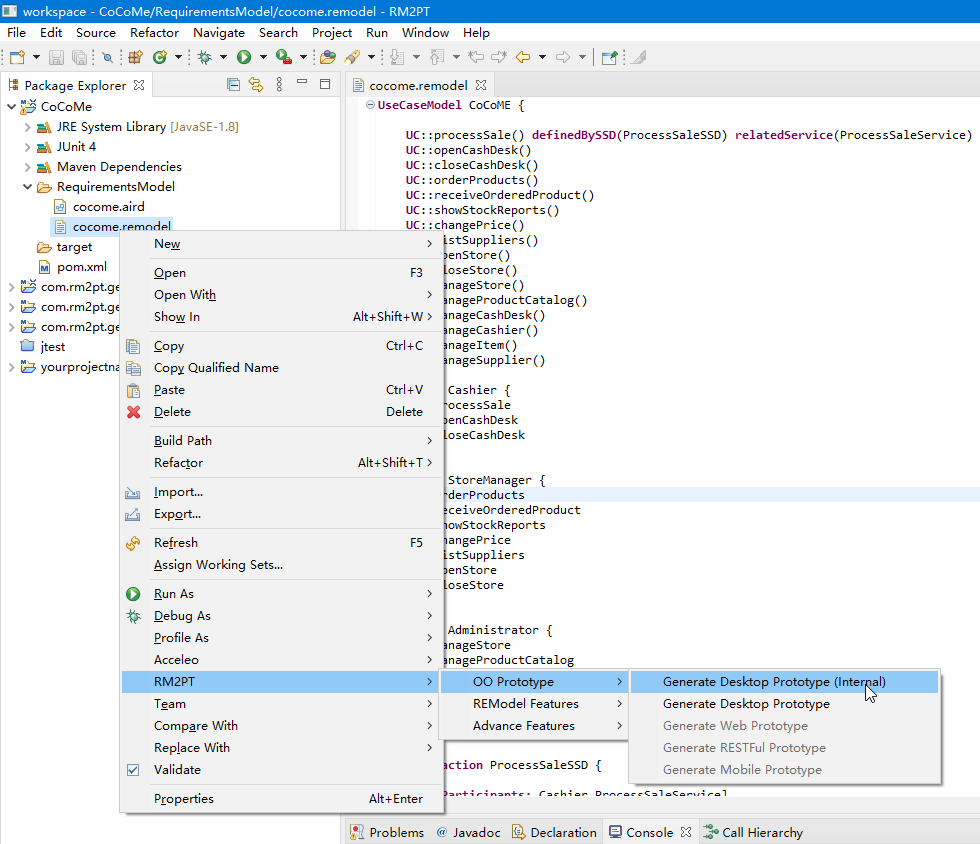
\includegraphics[width=0.7\linewidth]{RM2PT-generate}
}
\onslide*<3>{
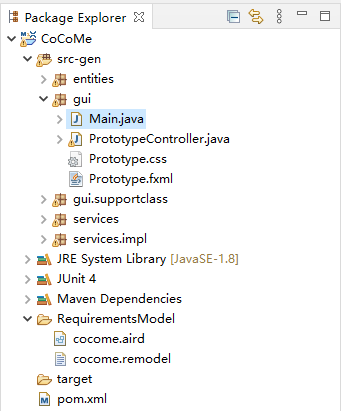
\includegraphics[width=0.5\linewidth]{rm2pt-folder-structure.png}
}
\onslide*<4>{
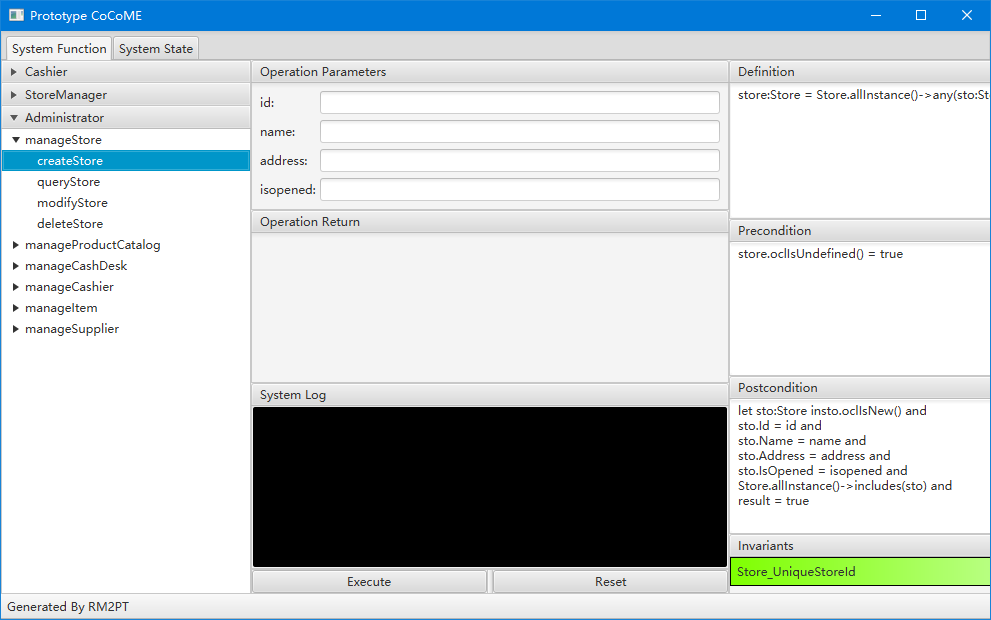
\includegraphics[width=\linewidth]{cocome-javafx.png}
}

\onslide<5>{
We contemplate to improve RM2PT so that it can generate smart contracts.
}

\end{frame}

\section{Literature Review}
\begin{frame}{Source Code Classification}

\begin{itemize}
\item \etal{Allamanis}~[] proposed the naturalness hypothesis.
\begin{itemize}
\item Programming languages are like natural languages to a great extent.
\end{itemize}

\item  More and more work in software engineering start to use neural networks.
\begin{itemize}
\item neural machine translation (NMT), transformers
\end{itemize}
\end{itemize}
\end{frame}

\begin{frame}{Neural Networks in Source Code Classification}


\begin{itemize}
\item  Grammformers~[] takes the context text and generates next code statements. The generated statements may contain holes.

\item \etal{Alexandru}~[] used NMT to annotate source code tokens with typing.

\item \textsc{JSNice}~[] predicts names of JavaScript identifiers and type annotations of variables.

\item \etal{Mou}~[] used a convolutional neural network to classify programs by functionalities.

\item detection of variable misuse~[],
bug localization~[],
API suggestion~[],
code completion~[]
\end{itemize}
\end{frame}

\begin{frame}{Datasets for Source Code Classification}
\begin{itemize}
\item \etal{Jiang}~[] collected a dataset of \num{1006} repositories from GitHub.
\begin{itemize}
\item unlabeled
\item mixed with Java and other languages
\end{itemize}

\item The dataset created by the authors of RMiner~[] comprises \num{3188} refactorings found in 538 commits from 185 projects.
\begin{itemize}
\item allow functional changes
\end{itemize}
\end{itemize}

\end{frame}



\begin{frame}{Smart Contracts~[]}

\begin{figure}
\centering
\begin{subfigure}[T]{0.3\textwidth}
	\includegraphics[width=\textwidth]{"smart contract architecture"}
	\caption{smart contract architecture model}
\end{subfigure}
\hfill
\begin{subfigure}[T]{0.65\textwidth}
	\includegraphics[width=\textwidth]{smart contract states.pdf}
	\caption{Finite-state of smart contract}
\end{subfigure}
\end{figure}


\end{frame}


%\begin{frame}{Duplicated Computing}
%\begin{itemize}
%\item Shae and Tsai~[] argue smart contracts are duplicated computing rather than distributed computing.
%\item<2-> They proposed a blockchain architecture for precision medicine.
%\begin{itemize}
%\item Smart contracts execute on chain.
%\item Applications run on a personal computer and call smart contracts
%\item Miners run the smart contract. The smart contract can be a Tensorflow program.
%\end{itemize}
%\end{itemize}
%\end{frame}

\begin{frame}{Distinctions between smart contract and OO languages}

\begin{itemize}
\item Reentrancy
	\begin{itemize}
	\item Smart contracts tend to call each other.
	\item The local states of one smart contract can only be modified by its own code.
	\end{itemize}

\item No multi-threading despite of attempts~[28,29]

\item \etal{Bram}~[20] holds that access control restrictions are a necessary part of the public specification of a contract.
\begin{itemize}
\item invented a DSL for Ethereum smart contract verification
\item not use Object Constraint Language (OCL)
\end{itemize}
\end{itemize}
\end{frame}


\begin{frame}{Transformation}

\begin{itemize}
\item State-of-the-art research is able to turn UML into fully executable code~[], including RM2PT.
\item RM2PT is able to complete 93.65\% of system operations.
\begin{itemize}
\item can check pre-conditions, post-conditions, and invariants
\item a runtime validation approach
\item<2-> These condition checking statements are transformed from OCL.
\item<3-> The language of the requirement document as a whole is unspecified.
\end{itemize}

\end{itemize}

\end{frame}

\begin{frame}{Verifying Smart Contract}
\onslide<+->
\begin{itemize}
\item Runtime Checking
\begin{itemize}
%\item<+-> RM2PT uses this approach.
\item<+-> ContractLarva~[] uses Dynamic Automata with Timers and Events. It allows users to supply pre- and post-conditions for Ethereum.
\item<+-> Solythesis~[] supports quantifiers, e.g., ``for all'', ``exists''. \onslide<+->{It invented delta update and delta check techniques so it doesn't have to suffix the checking statements to every transaction.}
\end{itemize}
\item[]<+-> {\color{Green} \checkmark} gain correctness or security guarantees
\item[]<.-> {\color{red} \texttimes} no longer Turing-complete


\item Static Analysis \onslide<+->{is hard.}
\begin{itemize}

\item<+-> formalize the requirements to a specification
\item<.-> abstract implementation to a formal mathematical model
\item<.-> check the model against the specification~[]
\item<+-> Securify~[] translates Solidity smart contract into Datalog and verifies security properties with a SMT solver.

\end{itemize}

\end{itemize}

\end{frame}


\begin{frame}[t]{Consensus Algorithm}
\begin{itemize}
\item The execution result of a smart contract must be in consensus to be added to the blockchain.

\onslide*<1>{
\begin{tikzpicture}[node distance=0.5cm and 1cm, scale=0.9, transform shape]
\node (application) [process] {application layer};
\node (execution) [process, below=of application] {execution layer};
\node (verification) [process, below=of execution] {verification layer};
\node (sm) [process, below=of verification] {smart contract layer};
\node (transmission) [process, below=of sm] {transmission layer};
\node (data) [process, below=of transmission] {data layer};

\draw [arrow] (application) -- (execution);
\draw [arrow] (execution) -- (verification);
\draw [arrow] (verification) -- (sm);
\draw [arrow] (sm) --  (transmission);
\draw [arrow] (transmission) -- (data);

\path[draw=red] (verification) circle [x radius=2cm, y radius=0.7cm];
\end{tikzpicture}
}

\begin{itemize}
\item<2-> Poof of Work, Poof of Stake, Practical Byzantine Fault Tolerance
\item<2-> A group of miners run the same piece of code to check if they got the same result.
\item<3-> Shae and Tsai~[19] calls it duplicated computing.
\end{itemize}

\item<3-> {[27]}~used communicating sequential processes and queuing theory to model the behavior of a consensus algorithm.
\end{itemize}

\end{frame}

\begin{frame}{Smart Contract Applications}
\begin{itemize}
\item CoCoME~[30] describes a trading system in a supermarket setting.
	\begin{itemize}
	\item a local, single-user system, no parallelism
	\item RM2PT is fully tested on CoCoME.
	\end{itemize}

\item SLEX-Web~[31] is a web application for school.
\item Dao~[32] implemented a Vietnamese certificates application called ECefblock running on Hyperledger Fabric.
	\begin{itemize}
	\item in MVC pattern
	\item has requirement documents
	\end{itemize}
\end{itemize}
\end{frame}

\section{Problem Formulation}

\begin{frame}{Tech Stack of Smart Contracts}
\onslide*<1>{
\begin{figure}
\centering
\includegraphics[width=\linewidth]{techstack}
\end{figure}
}

\onslide*<2->{
\begin{itemize}
\item Hyperledger Fabric
\item Java
\item on-chain
\item pBFT
\end{itemize}
}


\end{frame}


\begin{frame}{Aims and Objectives}

Identification\\
\begin{itemize}
\item study characteristics of blockchains and smart contracts
\item find out which functional implementations are transformable
%in MVC, no multi-threading
\item train classification neural networks to identify these patterns
\end{itemize}

Transformation\\
\begin{itemize}
\item transform source code to HyperLedger Java
\item add static analysis or runtime checking
\item find a model to formally describe the smart contract
	\begin{itemize}
	\item rCOS~[34] for component-based software
	\item partial order by refinement calculus
	\end{itemize}
\end{itemize}

\end{frame}

\begin{frame}{Relevance, Novelty and Originality}
\begin{itemize}
\item The use of neural network in program analysis is lacking.
\item The transformation rules encoded in RM2PT are manually devised without much theory support.
\item I will use neural network.
\begin{itemize}
\item No need for a rigid syntax parser
\item Neural network delivers a percentage
\item Extend RM2PT to generate smart contract applications
\end{itemize}
\end{itemize}


\end{frame}




\begin{frame}{References}
See the paper
\end{frame}

%
%{
%	\usebackgroundtemplate{\includegraphics[height=\paperheight]{fixie.jpg}}%
%	\contourlength{.06em}
%	\begin{frame}
%	\onslide<2->
%	\begin{tikzpicture}[overlay]
%	\node[yshift=1cm] at (current page.center) {\contour{white}{\Huge Thank you!}};
%	\end{tikzpicture}
%	\end{frame}
%}

\end{document}
